\documentclass[a4paper]{article}

%% Language and font encodings
\usepackage[english]{babel}
\usepackage[utf8]{inputenc}
\usepackage[T1]{fontenc}
\usepackage{graphicx}
\usepackage{subcaption}


%% Sets page size and margins
\usepackage[a4paper,top=3cm,bottom=2cm,left=3cm,right=3cm,marginparwidth=1.75cm]{geometry}

%% Useful packages
\usepackage{amsmath}
\usepackage{graphicx}
\usepackage[colorinlistoftodos]{todonotes}
\usepackage[colorlinks=true, allcolors=blue]{hyperref}

\title{Reporte de Actividad 2: Introducción a Phyton, Jupyter y Pandas}
\author{Jesús Antonio González Espinosa \\ \\ Física Computacional 1}
\date{7 de Febrero del 2018}

\begin{document}
\maketitle

La segunda actividad del curso fue usar un ejemplo aportado por el profesor para empezar a identificar e interpretar el lenguaje de programación Python, en el entorno de Jupyter Notebook. También, en base al mismo código, se nos pidió realizar unas actividades más que seguían con el contenido del ejemplo dado. Ambas partes de la actividad fueron con el objetivo de introducirnos al uso de lenguaje de programación Python en el entorno Jupyter Notebook. 

\section{Introducción}

\subsection{¿Qué es Python?}
Python es un lenguaje de programación interpretado, o sea, que el código no requiere ser compilado, ya que consiste en ser interpretado en tiempo real. Además, Python es multiparadigma, al permitir varios estilos de programación como programación orientada a objetos, programación imperativa, programación funcional, o muchos otros que son soportados mediante el uso de extensiones. Además, uno de los beneficios de él, es que tiene una sintaxis muy accesible, haciendolo fácil de escribir y leer. Otra de las ventajas de Python es que al ser de licencia de código abierto, hay una gran comunidad que crea librerias que aportan herramientas extras.

\subsection{¿Qué es Jupyter Notebook?}
Antes de hablar de Jupyter, es necesario conocer los documentos "notebook". Estos son documentos que contienen tanto código como elementos de texto, con el fin de dar provecho de ambos en conjunto. 
Jupyter Notebook es una aplicación que permite editar y correr documentos notebook en exploradores web. No requiere tener acceso a internet para trabajar en él. Al entrar a la aplicación, este te presenta un tablero o panel de contro, donde se muestran todos los archivos locales, que permite abrir los documentos tipo notebooks. Hoy en día soporta muchos tipos de lenguajes de programación. 

\section{Actividad}
En esta actividad usamos Jupyter Notebook para trabajar con Python. Lo que haremos es usar un documento de Jupyter Notebook de ejemplo que tiene una códigos en Python que dan descripción y presentación de varias tablas de datos de una estación del Servicio Meteorológico Nacional; el cual vamos a replicar pero con una nueva estación meteorológica. En este caso, vamos a trabajar con los datos obtenidos por la estación ubicada en el volcán "La Malinche", en Tlaxcala. 

Se presentará un poco sobre los comandos y las librerías usadas durante la actividad y la función que tienen.

\subsection{Comandos}

Al iniciar, lo primero que se hace es abrir las bibliotecas necesarias para el trabajo. En éste caso, se usaron tres, y se les asigno a una variable. Fueron llamadas por el código:

\begin{center}
\textit{import pandas as pd \\ import numpy as np \\ import matplotlib.pyplot as plt}
\end{center}

\begin{itemize}
\item \textbf{Pandas:} es una bibloteca destinada al análisis de datos, que proporcina estructuras de datos flexibles y permite trabajar con ellos de manera muy eficiente. 
\item \textbf{Numpy:} una biblioteca de funciones matemáticas de alto nivel para operar con esos vectores o matrices
\item \textbf{Matplotlib.pyplot:}  biblioteca para la generación de gráficos a partir de datos contenidos en listas o arrays
\end{itemize}

\bigskip

Con las librerias listas, se cargaron los datos meteorológicos de "La Malinche" mediante el comando: 
\begin{center}
\textit{df0 = pd.read\_csv('LaMalinche.txt', skiprows=4, sep='\char`\\ s+')}
\end{center}
Con esto, ya se puede trabajar con los datos. Dentro del archivo ejemplo hay varios comandos que presentan varios análisis de los datos. Algunos comandos fueron \textit{df0.head()}, que presenta tanta cantidad de datos del archivo como pongas entre el paréntesis. También usamos los comandos \textit{df = pd.DataFrame(df0)}, en conjunto con \textit{df = dtypes}, el primero siendo para dar estructura de data frame a los datos, y el segundo para presentar los tipos de datos que Pandas ha reconocido.

\begin{figure}[h!]
  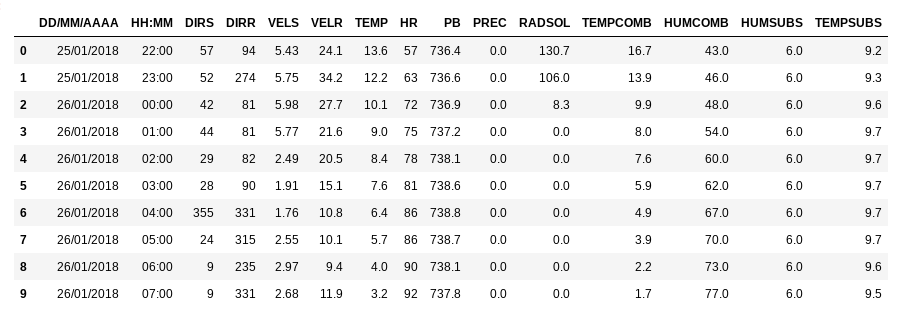
\includegraphics[width=\linewidth]{Tabla_dfHead.png}
  \caption{Datos del archivo leído.}
\end{figure}

\begin{figure}[h!]
  \centering
  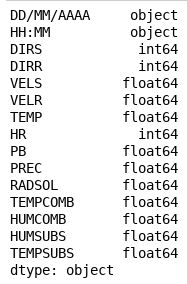
\includegraphics[width=0.3\linewidth]{Tabla_dfTypes.png}
  \caption{Tipo de datos del archivo.}
\end{figure}

Luego, en el ejemplo hay un código que une la columna de 'DD/MM/AAAA' con la de 'HH:MM', para poder crear una variable de tiempo única. Mostrando el código que hace el cambio de unificar y borrar las columnas, para crear una nueva llamada fecha: 
\begin{figure}[h!]
  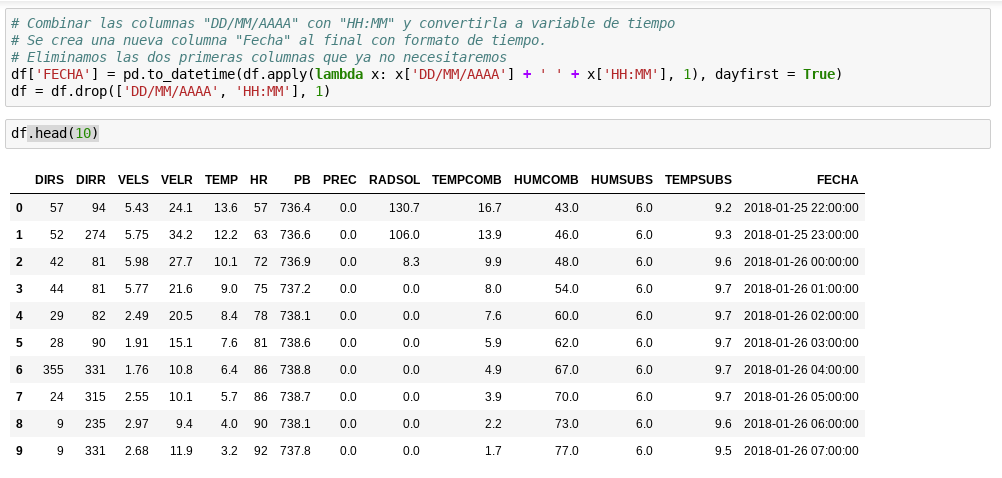
\includegraphics[width=\linewidth]{Tabla_dfHead2.png}
  \caption{Datos del archivo con los datos de la fecha unificados.}
\end{figure}

A partir de aquí, el código ejemplo muestra algunas herramientas como comandos para hacer análisis exploratorios o para sacar los promedios. En el ejemplo, se muestra el comando que hace el análisis exploratorio de los datos: 
\begin{figure}[h!]
  \centering
  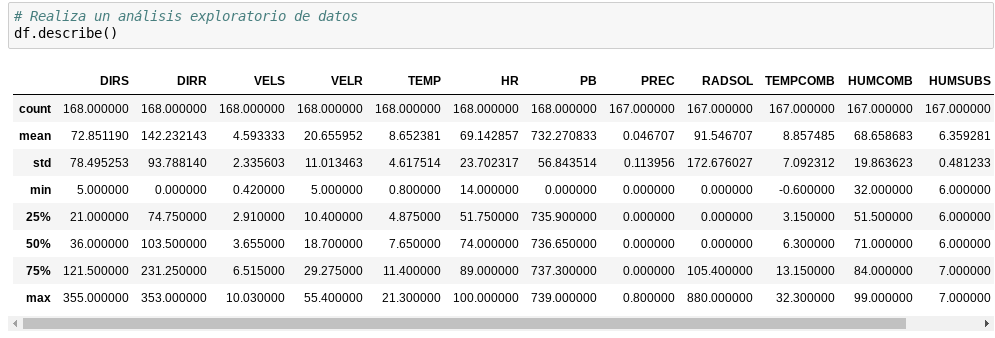
\includegraphics[width=0.3\linewidth]{df_Describe.png}
  \caption{Comando que muestra el análisis exploratorio de los datos.}
\end{figure}

También se muestran algunas formas de crear restricciones a los datos.

\begin{figure}[h!]
  \centering
  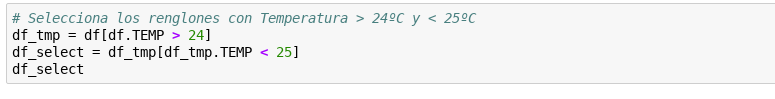
\includegraphics[width=0.3\linewidth]{df_tmp.png}
  \caption{Comando que hace restricciones.}
\end{figure}

En el caso de los datos de "La Malinche", no había datos que cumplían las restricciones, por lo que no hubo tabla para mostrar. 

Lo último que se mostró en el ejemplo, fueron como hacer gráficas. Se presentaron varias gráficas de acuerdo a los datos de "La Malinche"; algunos incluso con respecto al tiempo. Algunas gráficas con sus respectivos códigos fueron:

\begin{figure}[h!]
  \centering
  \begin{subfigure}[b]{0.3\linewidth}
    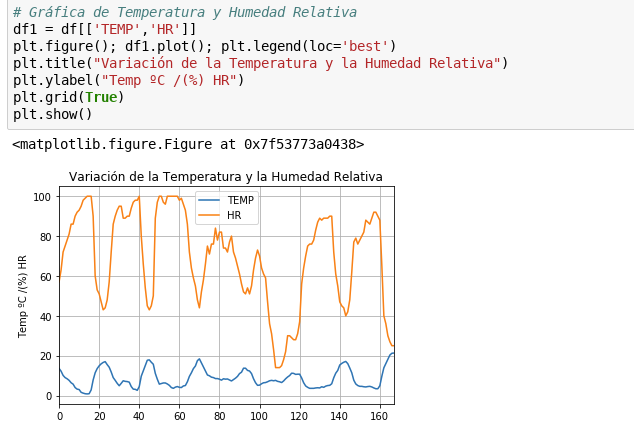
\includegraphics[width=\linewidth]{grafica2.png}
    \caption{Temperatura y Humedad Relativa}
  \end{subfigure}
  \begin{subfigure}[b]{0.3\linewidth}
    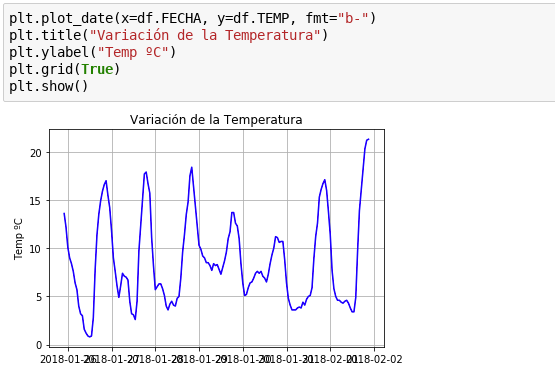
\includegraphics[width=\linewidth]{grafica3.png}
    \caption{Variación de Temperatura}
  \end{subfigure}
  \caption{Gráficas de los datos de La Malinche}
\end{figure}

Esto dio fin al ejemplo e inicio a una actividad para el alumno en el cual en base al código de ejemplo, debíamos lograr obtener más gráficas y análisis de datos.

\subsection{Actividad Adicional}
\begin{enumerate}
\item\textbf{Crear una gráfica que muestre la rapidez de los vientos y la rapidez de las ráfagas, como funciones del tiempo. ¿Cuáles son las horas del día con más viento?}

Para esta gráfica use pedazos de código de los ejemplos anteriores, un pedazo fue de la gráfica de "Variación de la Temperatura y la Humedad Relativa" para usar dos gráficas en una; y el otro pedazo fue de la gráfica de la "Variación de la Temperatura" para hacerla con respecto al tiempo. Finalmente, limite el tiempo a un día, para poder ver las horas del día con más viento. Podemos notar que alrededor de la media noche, se da el pico más alto en la gráfica del viento, ya que se ve entre las 21 horas y el inicio del día 30.

\begin{figure}[h!]
  \centering
  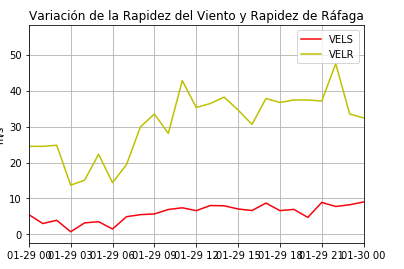
\includegraphics[width=0.6\linewidth]{ActGraf1.png}
  \caption{Gráfica de Velocidad de los Vientos y Rapidez de las Ráfagas.}
\end{figure}


\item\textbf{Crear una gráfica con la dirección de los vientos como función del tiempo y comentar sobre los vientos dominantes en el sitio de estudio.}

En la gráfica podemos ver que está muy variado, pero se puede notar fácilmente que en varios días la dirección domina en 0 grados. 

\begin{figure}[h!]
  \centering
  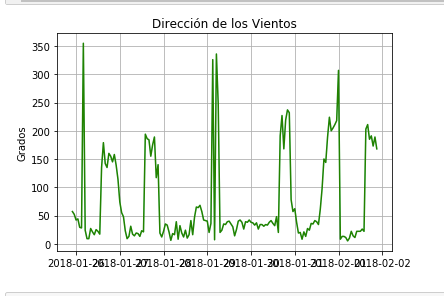
\includegraphics[width=0.6\linewidth]{ActGraf2.png}
  \caption{Gráfica de la Dirección de los Vientos.}
\end{figure}


\item\textbf{Muestre el comportamiento de la Radiación Solar como función del tiempo. ¿Que puedes comentar?}

Esta gráfica la limite a un solo día para poder observar el comportamiento del sol durante el día. Podemos ver que muestra en la gráfica radiación solar durante la noche. Esto puede ser a causa de problemas con la adaptación del uso horario en el código, o de alguna manera llega la radiación solar a esa zona en la noche. 

\begin{figure}[h!]
  \centering
  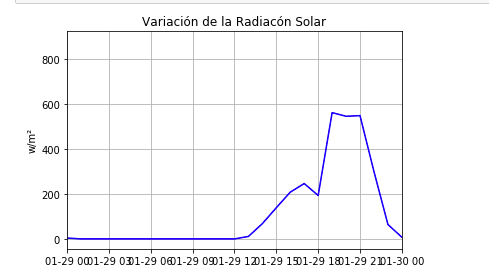
\includegraphics[width=0.6\linewidth]{ActGraf3.png}
  \caption{Gráfica de la Radiación Solar.}
\end{figure}


\item\textbf{¿Cuál es el lapso de temperatura diaria? (Diferencia entre la temperatura máxima y la mínima).}

Ahora para poder ver el lapso de temperatura diaria, se limitó el rango a un solo día, basado en el ejemplo,y con eso, se evaluo la temperatura máxima y mínima con comandos que buscan esos datos específicos. Luego se depositaron en una variable, y luego se hizo la resta de ambos, para ver el lappso de temperatura, resultando en 6.1 Grados Centigrados. 

\begin{figure}[h!]
  \centering
  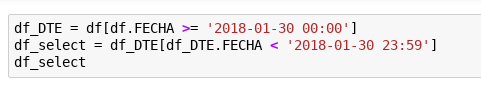
\includegraphics[width=0.2\linewidth]{ActGraf41.png}
  \caption{Código para limitar los datos a un día.}
\end{figure}
\begin{figure}[h!]
  \centering
  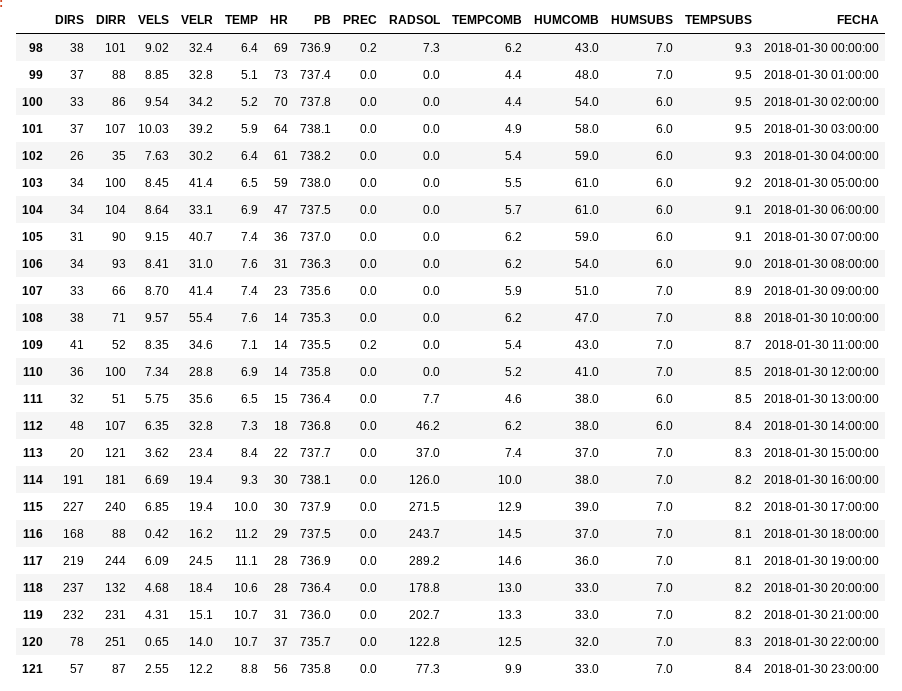
\includegraphics[width=0.2\linewidth]{ActGraf42.png}
  \caption{Mostrando los datos de un solo día.}
\end{figure}
\begin{figure}[h!]
  \centering
  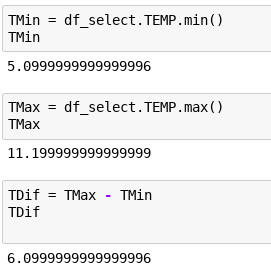
\includegraphics[width=0.4\linewidth]{ActGraf43.png}
  \caption{Diferencia entre Temperatura máxima y mínima.}
\end{figure}

\bigskip

\item\textbf{¿Puedes comentar sobre la relación entre la temperatura y la humedad relativa?}

Viendo la gráfica de Variación de la Temperatura y la Humedad Relativa, podemos inferir que cada vez que la temperatura sube, la humedad va a bajar, y viceversa. En otras palabras, son inversas una a la otra.

\begin{figure}[h!]
  \centering
  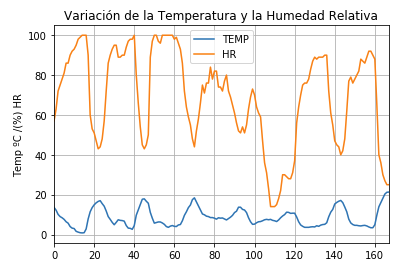
\includegraphics[width=0.6\linewidth]{ActGraf5.png}
  \caption{Gráfica de Temperatura y Humedad Relativa.}
\end{figure}

\item\textbf{Realiza el análisis exploratorio de datos, que resuma el sitio estudiado (Usar la función describe() sobre tu data frame.}

Los resultados del análisis exploratorio fueron:
\begin{figure}[h!]
  \centering
  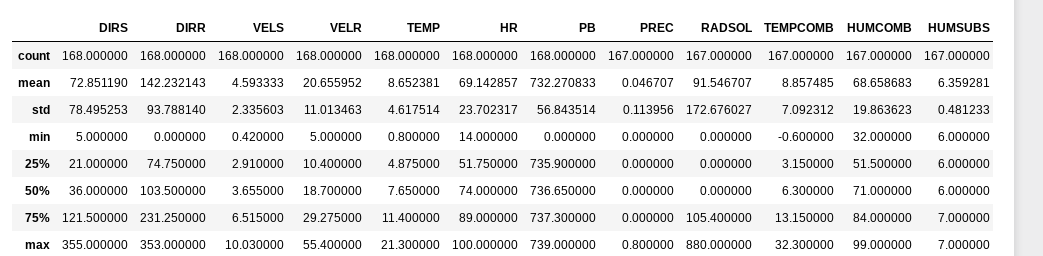
\includegraphics[width=0.6\linewidth]{ActExplor.png}
  \caption{Tabla de análisis exploratorio de los dato.}
\end{figure}

\section{Apéndice}
\begin{enumerate}
\item \textbf{¿Cuál es tu primera impresión de Jupyter Notebook?}

Ha sido interesante conocer éste nuevo entorno de programación y la forma en la que trabaja. Me impresiona y me es agradable poder correr cada línea a mi gusto, ya que anteriormente la única forma que conocía para correr códigos era con FORTRAN y era compilar cada vez que querías correr el programa lo cual se podía poner tedioso. 
\item \textbf{¿Se te dificultó leer código en Python?}

Al principio sí, ya que es un nuevo lenguaje que no conozco nada, pero mediante le fui buscando y moviendo a las líneas de código y buscando en Internet, las cosas empezaron a tomar sentido. 
\item \textbf{¿En base a tu experiencia de programación en Fortran, que te parece el entorno de trabajar en Python?}

Es mucho más sencillo, ya que no hay que estar haciendo cosas como compilar cada vez que quieres probar tu código. También siento mayor rapidez al entender los códigos, tal vez sea porque FORTRAN fue el primer lenguaje de programación que aprendí, pero a pesar de eso, siento una mayor comodidad desde un inicio al trabajar con Python.
\item \textbf{A diferencia de Fortran, ahora se producen las gráficas utilizando la biblioteca Matplotlib. ¿Cómo fue tu experiencia?}

Es impresionante, ya que a tres semanas del curso ya estamos pudimos ver como graficar, ya que con FORTRAN en un semestre, nunca creamos una gráfica en si. 
\item \textbf{En general, ¿qué te pereció el entorno de trabajo en Python?}

Ha sido interesante, había escuchado mucho del lenguaje, pero nunca lo había trabajado, y ahora que lo hice, fue interesante notar que cuando dicen que es muy fácil de entender, veo que tienen razón, es muy directo en cuanto a sus comandos y Jupyter Notebook lo hace todavía más atractivo a la vista.
\item \textbf{¿Qué opinas de la actividad? ¿Estuvo compleja? ¿Mucho material nuevo? ¿Que le faltó o que le sobró? ¿Qué modificarías para mejorar?}

El salto que hubo del ejemplo a la Actividad Adicional fue algo que sentí muy pesado al inicio, no sabía que era lo que tenía que lograr o por donde empezar, pero después de volver a analizar los datos y buscar en Internet sobre los comandos, fue creando un mejor acercamiento, después de unos cuantos minutos ya me sentí más seguro en que no era algo difícil; al finalizarla, se puede decir que fue un poquito difícil, pero es algo que sí se puede lograr. La actividad fue una buena introducción a ambos Python y Jupyter Notebook.
\item \textbf{¿Comentarios adicionales que desees compartir?}

Hasta el momento, hubo mucha comodidad trabajando con Python, no sentí la misma presión que sentí cuando aprendí Python. Tal vez sea porque es el segundo lenguaje que estamos aprendiendo, pero espero que lo que dicen de que Python es un lenguaje muy sencillo y elegante.
\end{enumerate}

\section{Conclusión}

Jupyter Notebook ha resultado ser muy interesante, la versatilidad que trae es mucha gracias a su capacidad de usar múltiples lenguajes de programación, también gracias a su capacidad de ser modificado y usar bibliotecas para abrir más posibilidades a los usuarios. Su interfaz también es muy agradable a la vista, además de que en lo personal sentí muy cómodo al estar trabajando en un explorador web. 
Por otra parte, las limitaciones de Jupyter Notebook parecen ser pocas, pero entre esas, está la dificultad del trabajo colaborativo, así como la incapacidad de recuperar una celda que se haya borrado si es que no se guardo correctamente.Existen otras pequeñas limitaciones pero, la comunidad siempre está a la vanguardia buscando mantenerlas muy pequeñas, esto gracias a otra bondad de este entorno, que es su código libre. 

\section{Biblografía}
Willems, K. (2016) \textit{Jupyter Notebook Tutorial: The Definitive Guide.} Recuperado el 5 de Febrero del 2018 desde https://www.datacamp.com/community/tutorials/tutorial-jupyter-notebook

\bigskip

Alouini, Y. (2017) \textit{What are the pros and cons of using Python Jupyter versus a normal Python development enviorment?}. Recuperado el 6 de Febrero del 2018 desde https://www.quora.com/What-are-the-pros-and-cons-of-using-Python-Jupyter-versus-a-normal-Python-development-environment

\bigskip

Wikipedia (s.f.) \textit{Python.} Recuperado el 6 de Febrero del 2018 desde https://es.wikipedia.org/wiki/Python

\bigskip

Ingargiola, A. (2015) \textit{What is the Jupyter Notebook?}. Recuperado el 6 de Febrero del 2018 desde http://jupyter\-notebook\-beginner\-guide.readthedocs.io/en/latest/what\_is\_jupyter.html




\end{enumerate}
\end{document}